% 3. Anatomical Models
\section{Anatomical Models}
\label{subsec:anatomical_models}

The structure of the internal lung is significantly influenced by the
hierarchical arrangement of the airways, which resemble a fractal
branching tree\cite{suki2011}. The design of this airway tree is
crucial for its function, as the branching pattern affects 
airflow and particle deposition. In modeling the human airway tree, it
is widely accepted that the airways follow an irregular dichotomy
pattern. Unlike regular dichotomy, where each branch splits into two
identical daughter branches, irregular dichotomy results in daughter
branches that can vary significantly in length and diameter.

\begin{figure}[H]\centering
  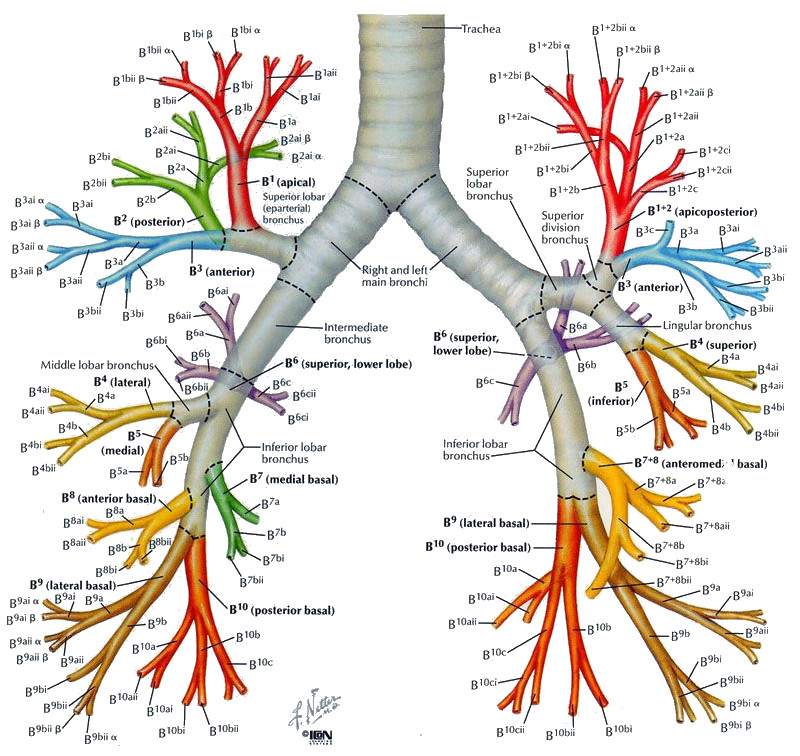
\includegraphics[width=.8\textwidth]{airway_tree_no_left_best.jpg}
  \caption{Representation of the major airways.}
  \label{fig:airway_tree_anatomical}
\end{figure}

% GESTISCI IMMAGINE E TESTO SOTTO
\begin{figure}[H]\centering
  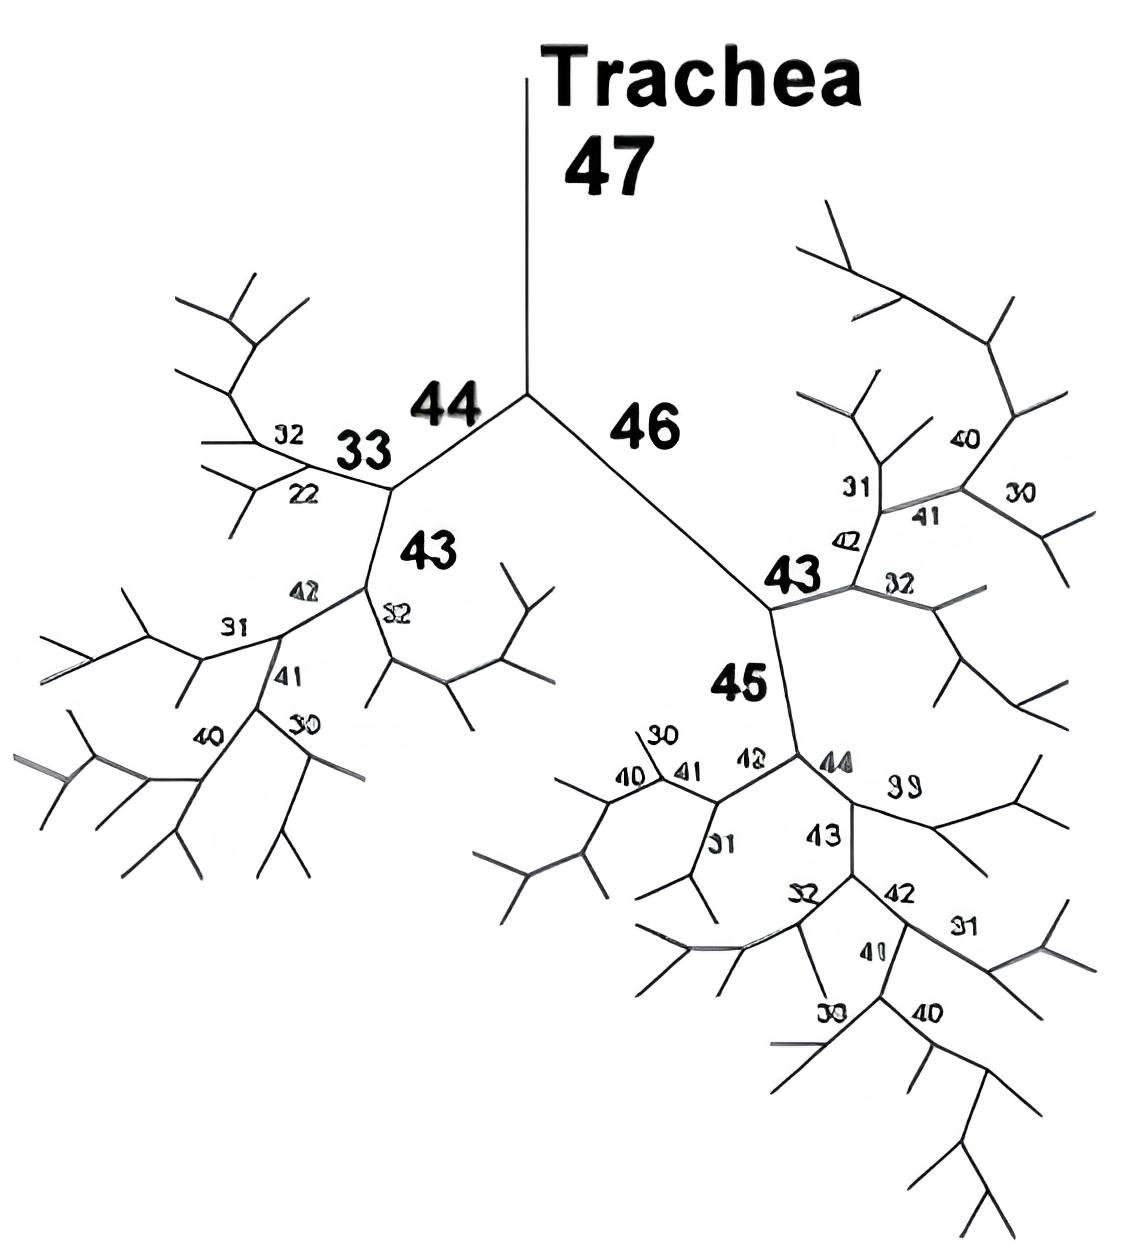
\includegraphics[width=.55\textwidth]{albero_dicotomico_best.png}
  \caption{The dichotomous bronchial tree.}
  \label{fig:albero_dicotomico_anatomical}
\end{figure}

% AGGIUNTA QUESTA MODIFICA, COMPLETARE
% -> spiegato il concetto in inglese.
\Cref{fig:albero_dicotomico_anatomical} serves as a reference for
constructing anatomically coherent adult lungs. In a dichotomous tree,
each airway (excluding the trachea) has a single parent branch and two
daughter branches (excluding the acini).  Asymmetrical bronchial trees
are a specific class presenting uneven splitting: Horsfield orders of
two siblings are different (causing recursion index $\Delta$
to exist, see \cref{fig:airway_impedance}).  Branching angles, lengths, and diameters can vary, thus resulting in different mechanical
properties.

Newborn lungs can be considered as having an analogous structure.

% LEGGERE INTRONORA E TAWHAI, POI CAPIRE COME CITARLI IN QUESTO PUNTO.
% Prima inserisco bene i modelli fregandomene se sono di adulti o
% neonati e poi dico cosa esiste in letteratura.  In questo punto devo inserire anche i parametri Rd, Rl ecc.

3D anatomical models have been generated from CTs by reconstructing
the missing distal airways through
algorithms\cite{tgavalekos2003,tawhai2000}.  Model consistency was
then studied, and its characteristics were compared with histological
measurements\cite{horsfield1987}.  Considering semilogarithmic plots
of the number of branches, lengths, and diameters against Strahler orders,
it is possible to define three important metrics:

\begin{description}
\item $R_{\text{b}}$: The branching ratio. It is defined as the
  antilog of the \emph{absolute value} of the slope of the number of
  branches. It is the factor by which the number of branches increases
  in successive orders \emph{down the tree}.
\item $R_{\text{d}}$: The diameter ratio. It is defined as the antilog
  of the slope of the diameters. It is the factor by which the
  diameter increases in successive orders \emph{up the tree}.
\item $R_{\text{l}}$: The length ratio.  It is defined as the antilog
  of the slope of the lengths.  It is the factor by which the length
  increases in successive orders \emph{up the tree}.
\end{description}


% {\color{red} MANCA QUESTA PARTE. Da tac, .. estratto centerline e
%   ricostruito con diversi algoritmi la parte mancante (Nora, Tawn..).

  % Dei modelli anatomici 3D sono stati realizzati a partire da tac di
  % pazienti, ricostruendo tramite algoritmi la parte mancante di albero
  % (cito Nora e Tawhai perchè modelli
  % diversi\cite{tgavalekos2003,tawhai2000} ).  La consistency del
  % modello è stata studiata confrontando le caratteristiche del modello
  % morfometrico dell'albero con quelle che sono state misurate sui cast
  % ex-vivo, in particolare nora dovrebbe citare cosa sono Rd, Rl ed Rb.
  % Copiare cosa sono questi valori (forse da Nora o Horsfield1987).
%   3D anatomical models have been generated from CTs by reconstructing
%   the missing distal airways through
%   algorithms\cite{tgavalekos2003,tawhai2000}.  Model consistency was
%   then studied, and its characteristics compared with histological
%   measurements.

%   Negli adulti e stato fatto un modello a partire della tac , più la
%   costruzione della parte mancante tramite algoritmi (citazione nora e
%   tawhai). e' stato poi verificato che i parametri morfo (le
%   dimensioni delle vie aeree generate) sono coerenti con quelli
%   ottenuti da misure istologiche. in particolare spiegare rl, rd, ed
%   rb.
% % Questa struttura in \Cref{fig:albero_dicotomico_anatomical} è stata
% usata come riferimento per la costruzione di alberi brochiali
% anatomicamanete coerenti per applicazioni su adulti. 

% PER CITARE NORA: \cite{tgavalekos2003}, PER CITARE TAWHAI
% \cite{tawhai2000}

Instead for infants, there exist models based on the
ovine\cite{al-jumaily2011} and canine\cite{herrmann2016} anatomy.

Mathematical models developed for adult lungs cannot simply be scaled
down to fit the lungs of newborns. Newborn lungs are not
simply one miniature version of adult lungs, but they present
significant differences in terms of bronchial branch proportions,
constituents of the airways\cite{merkus1996}, morphometric
characteristics ($R_{\text{d}}$, $R_{\text{l}}$,
$R_{\text{b}}$)\cite{horsfield1987} and composition\cite{hislop1989}.

%% Citare qui i riferimenti che ha fatto chiara nella call del 21.06
\textcite{mani2020} considered an adult lung model linearly scaled to
match newborn anatomical features.  The advantage of this approach is
that it respects the dimensions of the trachea and bronchioles. It doesn't
guarantee that the morphometric characteristics of the entire airway
tree are respected.  In this work, a few airway generation
parameters can be adapted, to better approximate
the target morphometric characteristics.

%%% Local Variables:
%%% mode: LaTeX
%%% TeX-master: "../Thesis"
%%% End:
